\documentclass{standalone}
\usepackage{arrayjobx}
\usepackage{xifthen}
\usepackage{tikz,textcomp}
\usepackage{ amssymb }

\begin{document}
	
\tikzset{ shorten <>/.style={ shorten >=0.2cm, shorten <=0.2cm } }

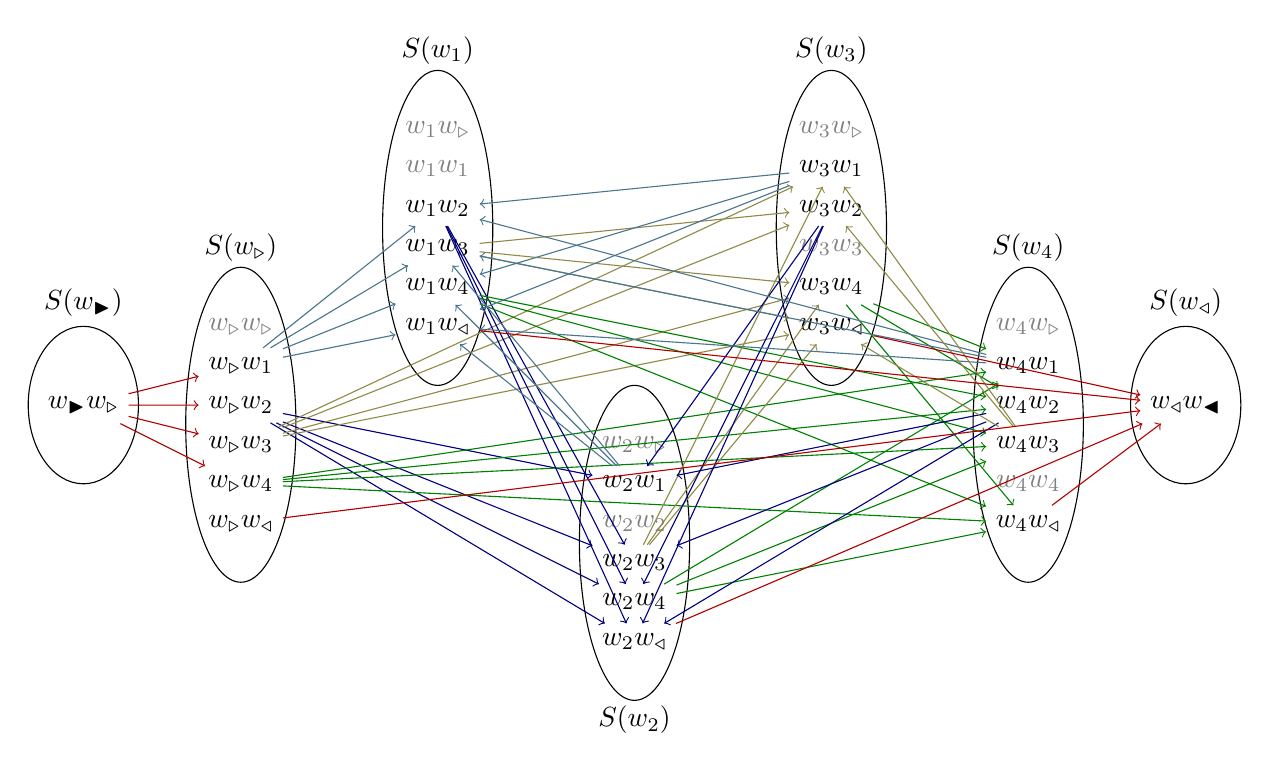
\begin{tikzpicture}
\newarray\Words
\readarray{Words}{$w_\triangleright$&$w_1$&$w_2$&$w_3$&$w_4$&$w_\triangleleft$}
\dataheight=5

\newcommand{\ystep}{0.5}

\newcommand{\gx}{}
\newcommand{\gy}{}


\newcommand{\drawgroupinner}{
	\foreach \j in {1,...,6}
	{
		\colorlet{MyColor}{black}%
		\ifthenelse{\i=\j}{\colorlet{MyColor}{gray}}{}
		\ifthenelse{\j=1}{\colorlet{MyColor}{gray}}{}
		
		\node[MyColor] (w_\i\j) at (\gx,\gy-\ystep*\j cm) {\Words(\i)\Words(\j)};
	}
	\draw (\gx,\gy-3.5*\ystep cm) ellipse (0.7cm and \ystep*4 cm);
}

\newcommand{\drawgrouptop}[3]{%
	\renewcommand{\i}{#1}
	\renewcommand{\gx}{#2 cm}
	\renewcommand{\gy}{#3 cm}
	\drawgroupinner{}	
	\node at (\gx,\gy+1*\ystep cm) {$S($\Words(\i)$)$};

}
\newcommand{\drawgroupbottom}[3]{%
	\renewcommand{\i}{#1}
	\renewcommand{\gx}{#2 cm}
	\renewcommand{\gy}{#3 cm}
	\drawgroupinner{}	
	\node at (\gx,\gy-8*\ystep cm) {$S($\Words(\i)$)$};	
}



\drawgrouptop{1}{0}{0}
\drawgrouptop{2}{2.5}{2.5}
\drawgroupbottom{3}{5}{-1.5}
\drawgrouptop{4}{7.5}{2.5}
\drawgrouptop{5}{10}{0}



\foreach \i in {1,...,5}
{	
	\foreach \j in {2,...,5}
	{
		\colorlet{MyColor}{black}%
		\ifthenelse{\j=2}{\colorlet{MyColor}{cyan!50!black}}
		{\ifthenelse{\j=3}{\colorlet{MyColor}{blue!50!black}}%
%		{\ifthenelse{\j=3}{\colorlet{MyColor}{red!50!black}}%
		{\ifthenelse{\j=4}{\colorlet{MyColor}{yellow!50!black}}%
		{\ifthenelse{\j=5}{\colorlet{MyColor}{green!50!black}}%
		{}}}}%}


		\ifthenelse{ \NOT \i=\j}{
			\foreach \k in {2,...,6}
			{
				\ifthenelse{\NOT \k=\i \AND \NOT \k=\j}
				{
					\draw[->,MyColor] (w_\i\j) -- (w_\j\k);
				}{}
			}
		}{}
	}
}

\node (w_S) at (-2cm,-1.5) {$w_\blacktriangleright$\Words(1)};
\draw (-2cm,-1.5) ellipse (0.7cm and 1 cm);
\node at (-2cm,-1.5cm +1.3 cm) {$S(w_\blacktriangleright)$};


\foreach \j in {2,...,5}
{
	\draw[->, red!70!black] (w_S)  --  (w_1\j);
}


\node (w_E) at (12cm,-1.5) {\Words(6)$w_\blacktriangleleft$};
\draw (12cm,-1.5) ellipse (0.7cm and 1 cm);
\node at (12cm,-1.5cm +1.3 cm) {$S($\Words(6)$)$};
\foreach \j in {1,...,5}
{
	\draw[->, red!70!black] (w_\j6) -- (w_E);
}

%\draw[->,line width=1mm,brown] (w_S) -- (w_12) -- (w_23)--(w_34)--(w_45)--(w_56)--(w_E);

\end{tikzpicture}

\end{document}